\chapter{研究现状}
\label{chap:intro}
\section{异常数据检测及相关方法}
随着科学技术的发展以及存储和计算能力的急剧增长,大数据的价值被日益体现了出来,数据挖掘技术被广泛地应用在了工业中和日常生活中。异常数据检测,作为数据挖掘算法中较为重要的一部分,引起了众多学者的关注和研究。本节介绍关于异常数据及其检测方法的相关内容。

异常数据是指在数据集中,不符合正常行为模式定义的数据模式\upcite{Chandola2009Anomaly},比如异常类或者反类。与正常模式的数据相比,异常数据在某些方面的特性不同,异常数据通常是少量存在的,也被称为离群点,所以异常数据检测也称为离群点检测。异常数据可以被分为以下三类\upcite{Chandola2009Anomaly},(1)点异常,如果一个单独的数据点与其他的数据点相比是异常的,这种情况被称为点异常,点异常是最简单的一种异常形式。(2)上下文相关异常,也被称为是条件异常\upcite{Song2007Conditional},上下文异常的数据,在全局看来可能不是异常的,但是从上下文的环境中看就是异常的,比如一年中每天的平均气温,假设十二月份的平均气温为零度,八月份的平均气温都为三十度左右,但是八月份某一天的平均气温只有零度,此时,从全局看,那一天的平均气温不是异常值,因为全年其它时间点有很多这样的值,可是从前后时间的温度来看,那一天的温度是异常的,这就是上下文相关异常的一个例子。上下文的环境一般由数据的某种属性来生成,比如语境属性和行为属性,上面举的例子中,一年中的某个时间就是数据的上下文属性,不同的时间下,数据点具有与时间属性相关的特性,这属于语境属性,而行为属性,是与数据产生者本身的行为有关系,比如全球的平均气温,不同地区的气温不同,气温与所在地区有关系,此时地区属性属于行为属性。(3)集体异常\upcite{Zheng2015Detecting},顾名思义,集体异常不是某个数据是异常的,而是一批数据都是异常的,而在这批异常数据中,单个的数据是不被检测为异常的,因为与它一起的数据同它具有一样的特性。这种情况可能发生在工业机器的传感器采集的数据中,当机器在运行中发生故障,一段时间后进行了修复,那么从故障发生的那一刻到修复好的那一段时间中,传感器采集的数据都是异常的,这就是集体异常。点异常是所有异常中最简单也出现最多的一种异常方式,现在学术界关于异常数据的研究大部分都是检测点异常的数据。 

异常数据检测方法可以分为基于监督的\upcite{G2013Toward,gonbadi2015supervised}和无监督的\upcite{Thakran2012Unsupervised}的方法。基于监督的异常数据检测方法的一种典型做法是,对正常数据分别进行学习和训练,建立一个正常数据行为模式,从而来进行异常数据的检测。而在有些数据集中,没有标记是否是异常数据,此时人工去进行标记类别是费时费力的,所以可以训练一个自适应的小模型,来对数据进行建模,从而检测异常数据,这就是无监督的异常数据检测。此外,异常数据检测方法可以分为基于统计的方法,基于聚类的方法,基于距离的方法和基于密度的方法,这些方法在下文中将会详细描述。

有关异常数据检测,一个重要问题是检测到的异常数据会以哪种形式输出出来,也就是检测后的输出是什么。一般来说,异常数据检测技术的输出有两种类型\upcite{Chandola2009Anomaly},分数型和标记型。分数型会输出测试数据集中的异常分数的序列,异常分数表示数据实例被认为是异常值的程度,所以可以设置一个阈值,比该阈值大的数据可被认为是异常数据。标记型则是对每一个数据实例添加一个类别标记,这种方式相对于分数型来讲,比较简单直接,但是精确度没有分数型高。本文采用的基于密度的LOF方法,就是采用的分数型输出方式。

目前比较常用的异常数据检测方法基本分为以下几类:基于统计的方法,基于聚类的方法,基于密度的方法和基于距离的方法等。
 
\subsection{基于统计的方法}
基于统计的方法\upcite{Ronald1995Outliers,Ozkan2016Online,Rousseeuw2017Anomaly}假设测试的数据集服从某个随机分布,为此数据集创建一个模型,然后通过不一致性测试来识别异常。数据的分布可以为正态分布,泊松分布,极值分布等等。

基于统计的学习方法是最早的异常数据检测方法,在1969年,Grubbs采用了基于统计的方法来检测单变量的异常数据\upcite{Grubbs1969Procedures},之后,Rousseeuw,Leroy和Barnett, Lewis进一步对基于统计的方法进行研究,提出了三倍偏差的方法\upcite{Gregory1987Robust,Barnett1978Outliers},即一组随机分布的数据,数值大部分分布在期望值减去3倍标准差和期望值加上三倍标准差这个区间之内,数据不在这个范围内的概率仅有不到$0.3\%$。因此可以设置阈值来更精确地检测异常数据,这在正态分布中,就是著名的$3\delta $准则。如图\ref{fig:fig2}所示是一个简单的基于统计的方法的例子,为了可视化方便,假设该数据X为一维数据,符合正态分布,记做$X\sim N\left(100,0.6 \right) $,其中$\mu = 100$为数学期望,$\delta ^{2}=0.6$为方差,则其概率分布图如图\ref{fig:fig2}所示,根据$3\delta $准则,可以设置两个阈值$\mu -3*\delta =97.879$,$\mu +3*\delta =102.121$,当数据点的值在$97.879$到$102.121$之间,则认为该数据是正常的,如果数据点的值小于$97.879$或者大于$102.121$,则认为数据是异常数据。

\begin{figure}
	\centering
	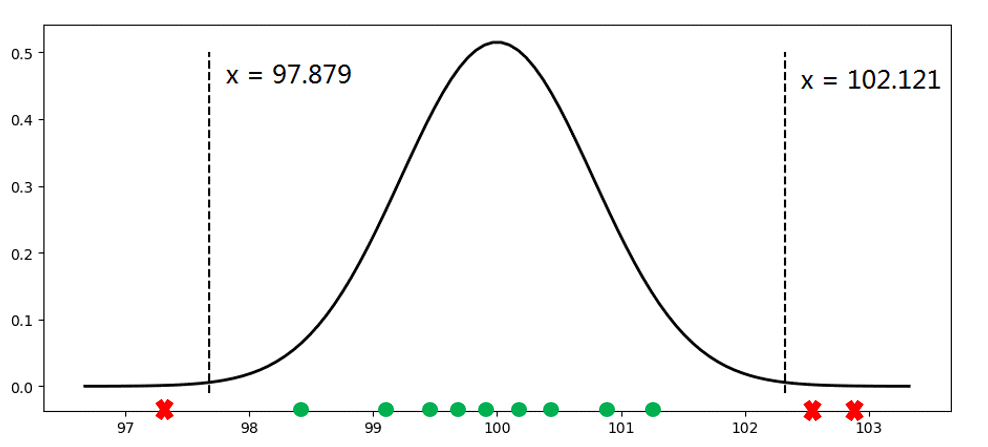
\includegraphics[width=0.75\textwidth]{figures/figure2x1}
	\caption{基于正态分布统计方法的异常数据检测}\label{fig:fig2}
\end{figure}

基于统计的方法建立在统计学基础上,对分布参数进行估计,当数据量充足而且检验类型已知的时候,这种方法能发挥很好的效果。但是在现实应用中,数据集一般不会完全符合某一种理想的数学分布方式,分布方式有时会随着时间的变化而发生改变,而且人们不清楚数据真正的分布情况,特别是在高维数据的情况下,很难去估测数据的分布,所以这种方式比较适用于低维的,知道数据分布方式的情况\upcite{金伟2016基于统计方法的异常数据检测及其修复}。

\subsection{基于聚类的方法}
基于聚类的方法\upcite{Rajasegarar2014Hyperspherical}是一种无监督的分类方法,聚类分析将数据集根据其相似性分为多个族群,数据点可以为测试集的向量值,或者是多维空间中的一个点\upcite{jain1999data}。直观地看,在使用聚类方法对数据集进行分类后,同一个族群中的数据点比其他类中的数据点更加相似。那么,在使用聚类方法对数据点进行分类后,如果在族群中的数据点,则与同一族群中的数据点相近相似,而不在分类的族群中的数据点,没有与其相近的点,根据异常数据点的定义,这些点可以看做是异常数据点。
 
基于聚类的异常数据检测方法根据某些假设,可以被分为三类\upcite{Chandola2009Anomaly}。(1)假设正常的数据点必定属于数据聚类后的集群,而异常数据点不属于任何集群。基于此假设的方法将已知的聚类算法应用到数据集上,然后对数据集进行聚类,从而得到不属于任何集群的数据点作为异常数据点。此类方法的优点是比较简单,可以直接使用已有的较为成熟的聚类算法,缺点是此类方法不是优先寻找异常数据点,而是将重点放在数据集的聚类上面,先将数据集聚类,分为多个集群,然后才能找到异常数据点。(2)假设正常的数据点是距离与其最接近的集群的形心较近的数据点,而异常数据点是距离与其最接近的集群的形心较远的数据点。基于此假设的方法需要先对数据集进行聚类,然后对每个数据点,计算它到距其最近的集群的形心的距离,以此距离作为判断其是否异常的参照。但是如果异常数据自成一个集群的话,此类方法不能很好地找出异常数据。(3)假设正常数据属于大的而且密集的集群,而属于小的或者稀疏的集群的数据点是异常数据。基于此假设的方法可以很好地解决异常数据自成一个集群的问题,它可以为集群的大小和密度设置阈值,集群的大小小于数量阈值或者集群密度小于密度阈值,即可将此集群中的数据点认为是异常数据点。

总的来说,基于聚类的异常数据检测方法\upcite{Zimmer2017Cluster}是一种典型的无监督的方法,不需要使用者了解数据本身,它可以适用于多种复杂数据类型的数据,具有较好的应用性,但是,这类方法的性能主要依赖与所选取的聚类算法,聚类算法的复杂度如果比较高,那么聚类算法很可能成为异常数据检测算法的性能瓶颈,而且,异常数据的检测只是聚类结果的“副产品”,如果异常点可以自身聚集成一个集群的话,或者异常点被分类到某个很大的集群的时候,这种方法就无法有效地检测异常数据。

\subsection{基于距离的方法}
为了解决异常数据检测方法在检测大数据集时,只能有效处理二维的或者只有两种属性的数据集的问题,1998年,Knorr和Ng最先提出了一种基于距离的方法\upcite{Knorr1998Algorithms,Knorr1999Finding}。他们提到,一个数据集$T$中的对象$O$,如果在数据集$T$中有至少$p$部分的对象与对象$O$的距离都大于$D$,那么就称对象$O$是$DB\left(p,D \right)$异常点,其中,$DB\left(p,D \right)$异常点是使用参数$p$和$D$的基于距离检测的异常点的简写。这种方法有效解决了当时只能处理低维的数据集的异常检测问题,可以适用于任意维度的数据集。并且,他们提出了几种简单的查找所有$DB\left(p,D \right)$异常点的算法,包括基于索引的算法,嵌套循环的算法,和基于单元的算法。

\textbf{基于索引的算法}:该方法将异常点的定义进行简化,定义一个异常点的$D$邻域内最多有$M$个点,则查找异常点的问题可以通过搜索每个对象的邻域解决。首先对数据集$T$建立多维索引结构,然后对每个对象$o$以半径$D$进行搜索,一旦在$D$邻域内搜索到$(M+1)$个对象,则停止搜索,并认定该对象$o$不是异常点,否则,$o$是个异常点。多维索引结构主要有$k-d$树\upcite{Bentley1975Multidimensional,Wald2006On},$R-$树\upcite{Guttman1984R, Hadjieleftheriou2016R}等,搜索一定范围内的时间复杂度的最好情况是$\Omega (N^{1-\frac{1}{k}})$,$k$是数据的维数,$N$是数据集的个数。当$k$增大时,搜索时间逼近$O(N)$。所以,查找所有的$DB(p,D)$异常点的时间复杂度为$O(kN^2)$。但是,这些时间只考虑了搜索的时间,没有考虑索引结构的建立的时间。实际上,索引结构的建立与维护是十分耗时的。

\textbf{嵌套循环的算法}:嵌套循环的算法可以避免基于索引的算法中建立索引结构的时间,它使用到了缓存,并将缓存分为两块,将整个数据集$T$分为多块。首先该算法将数据块读到第一个缓存中,对于其中某个数据点$t_i$,将其属性值$count(t_i)$赋值为0,计算其与其它数据点$t_j$的距离,如果$dist(t_i, t_j) \leq D$,则$count(t_i)$做加$1$操作,如果$count(t_i) > M$,则将$t_i$标注为正常的数据点,并且计算下一个数据点。否则,将其它数据块依次读入到第二个缓存中,依次计算两个缓存中数据的距离,直到全部数据块都计算过之后,第一个缓存中没有被标注的数据点就为异常数据点。该算法的时间复杂度为$O(kN^2)$。

\textbf{基于单元的算法}:该算法将数据集的属性值空间划分为边长为$l=\frac{D}{2\sqrt{k}}$的超立方体,$k$为数据的维数,每个立方体称为一个单元,然后将数据集中的数据点映射到单元中。每个单元$C$有两层邻居单元,第一层$L_1$为紧邻$C$的一层单元格,第二层为紧邻$L_1$的外部的$\left \lceil 2\sqrt{k} -1 \right \rceil$层单元格。如图\ref{fig:fig22}所示,是$k=2$时的单元$C$及其$L_1,L_2$层的示意图。每个超立方体的边长为$l=\frac{D}{2\sqrt{k}}$,则每个超立方体中的任意两个数据点的距离最长为$\sqrt{k}l = \frac{D}{2}$,两个相邻单元中任意两个数据点的距离最长为$D$,则单元$C$中的数据点与$L_1$层中的数据点的距离都不超过$D$。而单元$C$中的任意数据点距离$L_2$层中任意数据点的最长距离最短是$(\left \lceil 2\sqrt{k} -1 \right \rceil + 1) * l \geq D$。也就是说,$L_1$层中的数据点与$C$中的数据点的距离一定小于等于$D$,而$L_1,L_2$层包含了所有与$C$中的任意数据点的距离小于等于$D$的数据点。根据这些几何性质,每次计算单元$C$中的数据点时,只对$L_1,L_2$层中的数据点进行搜索计算即可。这种方法相当于对数据集进行剪枝,减少了计算量,提高了异常数据检测的效率。该算法的时间复杂度为$O(m(2\left \lceil 2\sqrt{k} \right \rceil +1)^k + N)$。

\begin{figure}
	\centering
	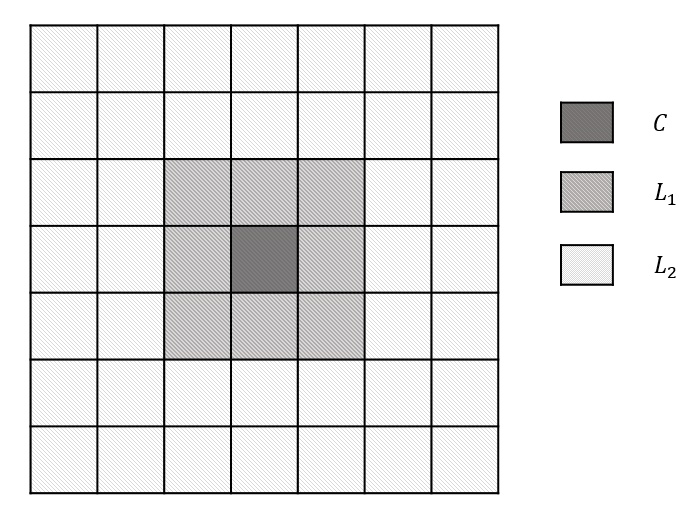
\includegraphics[width=0.45\textwidth]{figures/figure2x2}
	\caption{维数为$2$时某单元$C$及其$L_1,L_2$层示意图}\label{fig:fig22}
\end{figure}

与基于统计的方法相比,基于距离的方法\upcite{Zhang2016A}可以很好地适用于不满足某种特定的行为模式的数据集,而且在数据空间的维数比较高的时候,基于距离的方法也可以很好地检测出异常数据。但是对于参数$p$和$D$的确定,目前没有好的规律和算法,对于不同密度的数据集,$D$的取值不同,结果也会很不相同,因此测试结果具有较大的不稳定性\upcite{王斌2009面向不确定感知数据的异常数据检测技术}。而且当数据的属性值为非数值时,两个数据点之间的距离无法直接计算,需要将属性值转换为数值。

\subsection{基于密度的方法}
之前提到的基于统计的方法和基于聚类的方法等,都是考虑全局数据的,而基于密度的异常数据检测方法\upcite{Zhao2016Density},是针对局部数据的,这种方法计算每个数据点的邻近的密度,如果一个数据点的邻近点比较稀疏,则认为该数据点为异常数据,如果一个数据点的邻近点比较稠密,则认为该数据点是正常的。常用的密度定义有两种,一种是距离某个对象$o$最近的$k$个点到$o$的距离和的平均值的倒数,即假设距离对象$o$最近的$k$个对象的集合为$S$,则对象$o$的密度为
\begin{equation}
\rho = 1 / \frac{\sum_{p\in S}d(o,p)}{k}
\end{equation}
如果距离和的平均值小,则密度高。另一种定义是距离对象$o$为$d$的范围内的所有对象的个数。如果$d$邻域内的对象多,则密度大,但是该定义中的参数$d$不好确定,参数$d$如果太小,则很多正常点的密度也小,如果$d$太大,则异常点的密度也大。比较常用的基于密度的检测方法是LOF算法,该算法为了精确找出异常因子,定义了对象的局部可达密度,而且不仅仅考虑计算对象的密度,还考虑计算对象的邻域内的对象的密度。该算法为每一个对象计算出局部异常因子,表示对象的异常程度。该算法在下一章会详细介绍。

\subsection{其他方法}
大部分的异常检测方法,比如基于聚类的方法,基于分类的方法等,都是构建正常数据的模型,以这个模型来检测其它的数据是否异常,这类方法主要有两个缺点,一是异常数据的检测不是靠异常数据的建模来检测的,而主要是靠正常数据的建模程度来优化的,正常数据的建模越好,异常数据的检测才能越成功。这样会导致异常数据的检测不如期待的好,可能会导致有些异常数据检测不出来,而有些正常数据会被误判定为异常数据。二是因为计算复杂度的影响,大部分方法在实际应用中局限于较低维度和小规模的数据。

异常数据有着“少而不同”的特征,也就是说,异常数据在数据集中是占很少一部分的,而且异常数据的行为模式、属性值与正常数据有着显著区别。这个特点是根据异常数据的定义得到的,异常数据也称为离群点,是数据集中明显偏离大部分数据的数据点,所以在数据集中的比重不大,而且属性值偏离常见属性值之外。基于异常数据的特性,刘飞和周志华提出了一种不需要检测正常数据,直接隔离异常数据的方法\upcite{Liu2009Isolation, Liu2012Isolation}。因为异常数据的“少且不同”的特点,异常数据是特别容易与其它数据分隔开的。异常数据“少”,所以更容易被分割开来,分割的路径也相对较短。异常数据“不同”,所以在早期的分割中,就与其它数据分离了,基于这些考虑,他们提出了Isolation Forest方法,简称为iForest,这种方法对于一个给定的数据集,构建一个iTree的组合,然后在iTree中表现的路径短的数据点被认为是异常数据。该方法的主要思想是根据异常数据的特征,结合了机器学习中的随机森林算法,对数据样本的属性值进行了随机选取,从而对样本空间进行了随机划分,对数据的隔离过程表示成了对一棵树的建立过程。由于树的建立是随机的,所以建立多棵树,来提高准确率。这种方法的输入参数有两个,分别为构造的树的数目和数据的采样大小。以下为该方法的详细介绍。

iTree定义:iTree是一棵二叉树,全称为Isolation Tree。如果T是iTree的一个结点,那么T要么是一个没有子结点的叶子结点,要么是有个两个子结点的内部结点,且这个内部结点包含一个属性$q$和一个分隔值$p$。

建立iTree的过程如下,给出一个包含$d$维数据的数据集,随机选择一个属性和该属性上的一个值,将数据集进行分类。依次迭代分类,停止的状态为达到树的高度,数据集只剩一个,或者在数据集中的所有数据的值都相同。一个数据点的路径长度定义为这个数据点从根结点被分隔到叶子结点时所走的树的深度。

具体过程定义如下:

1.从原始数据集中随机选取数据,得到一个子数据集,作为根结点;

2.随机指定一个维度,选择该维度上的一个数作为切割点,在此维度上将数据划分为两类,作为两个子结点;

3.依次对子结点进行维度选择和切割,再生成子结点,直至树的高度达到一定值,或者子结点中只有一个数据值,或者子结点中的数据值都一样。此时,得到iTree;

4.以上过程进行$t$次,得到$t$棵iTree。

此时,可以设置一个阈值,如果一个数据点在多棵iTree上的路径长度低于此阈值,则认定该数据点为异常数据。

与其他常见方法相比,iForest方法的优点在于,采用了集成学习的思想,学习器由多个个体学习器构成,而且检测起来特别灵活,不需要构造正常数据的全部模型,只需要构建部分模型即可。iForest方法中,没有距离和密度的计算,可以减少了大量的计算工作。该方法是线性复杂的,内存要求也很低,这对于大规模数据的计算有着很大的优势。而且该方法适合于部署在大规模分布式系统上进行加速运算,因为每棵树都是相互独立的。且树的数量越多,该算法越稳定。但是该方法是随机选取维度,很多维度的信息都没有使用,也会有噪音维度影响精度,如果树的数目较少,算法可靠性必定会降低,而且该方法对全局的异常点检测比较准确,但是对于局部的相对稀疏点,检测可靠度较低。

\section{数据压缩及相关方法}
由上一章可知,时序数据是最常见的数据流模型之一。时序数据在多个行业中都有应用,如股票金融业中每日股票的开盘价最高价等序列值,天气气象中每日气温降雨量等序列值,工业中电网每日的流量等等。大数据时代,数据流的数量庞大,直接对原始数据进行存储难度较大,容易造成昂贵的存储代价和传输代价,且大数据的数据量大,价值密度低,大多数情况下,都只关注数据整体的特性和发展的趋势,没有必要对每个数据进行存储。所以,在保留数据的主体的特性的前提下,对数据进行模式表示,可以对原始数据进行压缩,减少存储空间和计算的代价,也可以保留数据的价值与特性,也有助于后续的数据分析与可视化,符合大多数应用领域的需求。

在流式环境下,时序数据成为随时间顺序不断增加的动态序列,可能具有无限的体积。而对流式数据进行处理时,如果将数据全部缓存起来再进行处理,需要大量的存储资源和计算资源,这是不可能的,所以需要在数据流入的同时对数据进行处理。在无法获知全局数据的情况下对数据进行压缩,如果数据处理不及时很可能造成数据丢失,因此,对计算效率提出了更高的要求。

时序数据的模式表示主要分为四类,分别有分段线性法,频域法,奇异值分解法和符号表示法。

\subsection{分段线性法}
分段线性法\upcite{Iijima1994A,Wang2016A},顾名思义,是先用算法将数据按照一定规律分段,然后在每段数据上,用线性函数对其进行拟合。该方法可以看做是用一系列不重叠的线段,近似地表达一条曲线。其中,最早出现的也是最简单的分段线性法是PAA方法,PAA方法将整体数据按照一定的长度平均分段,每段的数据用该段数据的平均值来表示。这种方法简单方便,但是比较粗糙,数据段与数据段之间不连续。之后的研究,为了解决这种问题,分别就分段与拟合两个方面,提出了多种不同的方法。

在数据分段方面,最简单的是平均分段,就是给定一个参数作为每段数据段的长度,对整体数据均匀分段。但是,平均分段不能很好地描述数据的特征,所以出现了非平均分段。非平均分段的算法有自顶向下算法,自底向上算法和滑动窗口算法,前两种算法是在静态数据整体上进行的,而滑动窗口算法可以在动态数据集上运行,支持在线分段。

自顶向下算法可以定义三个参数,分别为每个分段的最大误差,整个时间序列的最大误差,和分段数。该算法首先需要扫整个数据集,根据分割后两段的误差都处于较小等条件找到最佳的分割点,然后将原始数据序列分割为两个子序列,此时计算子序列的拟合误差,如果子序列的拟合误差小于误差阈值,则停止划分,否则继续划分子序列,直至所有的子序列的拟合误差都小于误差阈值。自底向上算法计算过程与自顶向下相反,该算法首先将整个数据序列划分为一个个相邻的短序列,这些短序列包含相邻的数据点,且拟合误差不超过阈值。将数据序列分为短序列后,计算相邻的序列合并后的拟合误差,将拟合误差最小的两个序列段合并,依次进行这个操作,直至任意相邻两段合并后的误差大于误差阈值。自底向上算法也可以人为定义每个分段的最大误差,整个序列的最大误差和分段数这三个参数。滑动窗口算法与前两种都不一样,它只可以定义每个分段的最大误差这一个参数,它的计算过程是有一个数据窗口,窗口中有一些相邻的数据点,如果窗口内的数据点的拟合误差小于阈值,则这个窗口增加窗口的宽度,同时接收新的数据点,并再次计算窗口内数据点的拟合误差,重复执行此操作直到窗口内的数据点的拟合误差大于阈值,此时该窗口内的数据为一个划分的数据段,并且开启一个新的窗口接收新的数据,开始下一个数据段的划分。在这些算法中,自顶向下算法算法时间复杂度最大,但是划分最为准确,不支持在线动态划分数据序列,自底向上算法也不支持在线动态划分数据序列,但是时间复杂度低,算法简单,精度介于其余两种方法之间。滑动窗口算法的划分效果最差,但是算法复杂度低,计算简单,而且具有在线划分的特性。所以,在选择算法时,应该结合应用场景和需求,选择最适合的算法。

每段数据的线段拟合分为两种,一种是直线插补法,直接将数据段的开始点和结束点用线段相连,作为该数据段的拟合线段,然后相邻段之间首尾相连,整个数据段被分为一系列连接的线段。一种是直线回归表示,这种方法通过最小二乘法拟合段内所有的原始数据,相邻段可以不连续,精确度更高,与原始数据更为接近,较为常用。

在这些基础上,国内外研究人员提出了许多更好分段和拟合的方法。为了更好地进行分段,许多方法将数据本身的特点作为划分依据,将整体数据序列划分为更适合本身趋势变化的数据段,如基于极值点的\upcite{张海涛2015时间序列的层次分段及相似性度量,戴爱明2009时间序列三角极值点线性分段算法},基于斜率的\upcite{刘贺红2010确定时间序列分段点的方法研究},基于特征点和趋势点的\upcite{Zhu2007A}方法。基于极值点的方法找到数据的极值点来作为分段点,但是这种方法划分容易过于精确而忽略了趋势加速点,但是其计算很简单,性能也比较好,而且不依赖于阈值。为了弥补其划分过于精确的缺点,可以设定一个距离阈值,加上判断,当两个相邻极值点的数据差不大于这个距离阈值时,只选择其中一个极值点,这种方法减少了极值点的数量,减少了分段的数量,被称为基于特征点的方法。趋势点是数据变化较大的点,包括极值点和趋势加速点和趋势减速点。基于趋势点的方法需要计算某点和相邻点的角度、弧度或者余弦等,将大于特定阈值的点称为趋势点。为了更好地拟合数据段,不仅仅局限于用线段来拟合数据段,而是可以用多种函数拟合数据段,如多项式函数,指数函数等多种曲线函数,曲线函数能更好地拟合数据的变化,线段表示其实就是多项式曲线表示的一种形式。

\subsection{其他方法}
频域法\upcite{Grinsted2004Application,Cooley1977The,Zhang2016An}是将一条时间序列看作是时间域上的一个信号,通过离散傅里叶变换\upcite{Dwivedi2015A}或者离散小波变换\upcite{Zhang2003Detection,Laisn2015A},将时间序列从时域空间映射到频域空间,将时域信号变换为频域信号。一个时间序列的时域信号可以看成各种周期扰动的叠加,时域分析只能反映信号的幅值随时间的变化的情况,很难表达出信号的频率组成和各频率分量的大小。而经过傅里叶变换,可以把任意的函数分解成为简单的周期函数的和,然后再将这些周期函数映射到频域内,此时,频域的自变量是频率,函数值为对应的振幅。频域分析可以确定各周期的振动能量的分配。

符号表示法\upcite{Lin2007Experiencing}的主要做法是将时间序列离散化,映射到由不同符号组成的符号空间,将时间序列表示为有限符号的有序集合。其过程如下,首先,将一个时序数列$X = \left \{ x_{1}, x_{2}, ..., x_{n} \right \}$进行$z-score$标准化,标准化式子为
\begin{equation}
q_{i}=\frac{\left ( x_{i}-mean\left ( X \right ) \right )}{std\left ( X \right )}
\end{equation},
其中$ i = 1, 2, … , n$,得到数列$Q = \left \{ q_{1}, q_{2},..., q_{n} \right \}$。然后对其进行平均分段,并且每一段用平均值表示,即
\begin{equation}
{q_{i}}^{'} = \frac{1}{k}\sum_{j=\left ( i-1 \right )k+1}^{ik}q_{j}
\end{equation},
得到序列$Q^{'}=\left \{{q_{1}}^{'}, {q_{2}}^{'}, ... , {q_{w}}^{'} \right \}$,其中$k$是压缩率,原长度为$n$,转换后的数列长度为$w$,$w = \frac{n}{k}$。然后得到这些离散的值后,将其映射到符号空间,转化为离散的符号。

奇异值分解法\upcite{Cadzow1983Singular}是一种基于统计概率分布的投影方法,可以对整个时序数据库进行整体表示。奇异值分解简称$SVD$,如果有一个矩阵$A$,对其进行奇异值分解,可以得到
\begin{equation}
A=U\Sigma V^T
\end{equation},
其中,假设矩阵$A$规模为$m\times n$,则矩阵$U$的规模为$m\times m$,矩阵$\Sigma$的规模为$m\times n$,矩阵$V^T$的规模为$n\times n$。矩阵$\Sigma$是一个对角矩阵,且对角元素从大到小排列,这些元素便是奇异值。由于排列在后面的许多对角元素接近于$0$,所以,可以只保留比较大的$r$个奇异值,即只保留矩阵$U$的前$r$列,矩阵$\sigma$的前$r$行前$r$列,矩阵$V^T$的前$r$行。所以,只需要保存三个比较小的矩阵,就可以表示一个大的矩阵,实现了数据的压缩。该方法多用于图像压缩方面。
\section{流式数据的处理}
上文提到的异常数据检测方法是用于静态数据集的方法,在进行检测前,数据集是完整的,可以对数据集进行多次的计算和分析。而流式数据一般具有数据量大,数据维度高,存储昂贵的特点,对流式数据进行异常数据检测,需要对上面提及的异常检测方法进行改进或者研究新的算法。目前,针对流式数据的异常数据检测方法的思想可以分为两类,第一类是对静态方法的改进,这类方法是最直接的一种方式,可以先创建缓存,积累一部分数据,对这部分数据进行训练,之后当新的数据到达时,对该数据进行检测,然后对模型进行更新和优化。该方法较为简单,但是如果流式数据有很大的动态变化,后来的数据的分布和行为模式发生很大改变,而模型是依据最前面的数据进行建模的,这种情况下该方法不能很好地检测后来的数据点。由此可见,该类方法适应性较差,比较适合数据的分布变化不是特别大的流式数据的检测。第二类是引入增量学习\upcite{He2011Incremental}和在线集成学习\upcite{Bifet2009Improving, Ando2015Ensemble}的思想,增量学习是指模型可以保留以前学习到的知识,并且不断地从新的数据中学到新的知识,集成学习是指不只构建一个模型,一个检测器,而是构建多个模型,然后从多个模型中检测到结果,最后将结果合成得到最终结果,上小节提到的iForest方法就是采用了集成学习的思想。这类方法相比与对静态方法的改进,可以很好地适用于数据分布变化很大的流式数据,具有很高的泛化能力。 

对流式数据进行异常数据检测的方法中,基于网格的方法\upcite{屠莉2009流数据的频繁项挖掘及聚类的关键技术研究}是常用的方法之一。基于网格的方法需要将数据点映射到网格中,计算网格的密度,当超过一定阈值时,认为这个网格是稠密网格,将相邻的稠密网格分成一类,网格密度小于一定阈值的网格则被认为是稀疏网格,当网格为稀疏网格时,可认为网格中的数据点为异常数据点。该方法可以满足流式数据“一次读取”的特征,每次数据点到来时只需要更新对应的网格的密度,处理速度较快,但是当数据的取值范围变大时,网格的数量也会变多,空间复杂度大大增加,此时进行异常数据的检测性能会下降。针对这个现象,相关文献中提到了改变网格划分,减少网格数量的方法。文献[62]%\cite{马菲2015一种基于可变网格划分的离群点检测算法}%
中,使用了可变网格划分的思想,先将数据的每一维等间距划分,然后比较相邻区间段的相似性,并将相似性高的相邻区间段进行合并。在文献[63]%\cite{王敬华2015基于粗约简和网格的离群点检测}
中,针对网格的每个维度的划分粒度小,会使网格数量显著地增加,而划分粒度大,又会使聚类精度不准确,异常数据检测的精度受到影响的问题,引入了属性维半径,提出了一种可变网格的划分方法,每一维根据不同的维半径划分。文献[64]%\cite{杨宜东2006基于动态网格的数据流离群点快速检测算法}
中,则提出一种动态划分网格的方法,首先生成初始网格,当网格的密度达到阈值的时候,选择方差最大的维度,将原网格划分为两个子网格,然后随着数据的逐步到来,对网格进行不断划分,直到一个合适的网格状态。但是基于网格的方法比较粗糙,精确度不高,当异常数据聚集时,容易认为其实正常的数据点。而一个聚类的外围数据点容易被认为是异常的。

\section{本章小结}
本章主要分为三部分,一部分介绍了异常数据检测的相关技术。首先介绍了异常数据的定义,异常数据的分类,以及异常数据检测方法的分类。然后,又从四个方面详细介绍了几种异常数据检测方法,分别有基于统计的方法,基于聚类的方法,基于距离的方法和基于密度的方法。最后,又介绍了工业上常用的iForest方法,并分析了该方法的优点与缺陷。第二部分介绍了现在的压缩算法,分别介绍了分段线性法,频域法,符号表示法和奇异值分解法的实现过程,并分析了三种分段方法,以及适用于流式数据压缩的滑动窗口算法。第三部分分析了当前的异常数据检测方法在流式数据上常用的方法。